% --------------------------------------------------------------
% This is all preamble stuff that you don't have to worry about.
% Head down to where it says "Start here"
% --------------------------------------------------------------

\documentclass[12pt]{article}

\usepackage[margin=1in]{geometry} 
\usepackage{amsmath,amsthm,amssymb}
\usepackage{color}
\usepackage{tikz, pgfplots}
\usepackage{graphicx}
\usepackage{epstopdf} %converting to PDF
\usepackage{subcaption}

\makeatletter

\renewcommand\section{\@startsection {section}{1}{\z@}%
	{-3.5ex \@plus -1ex \@minus -.2ex}%
	{2.3ex \@plus.2ex}%
	{\normalfont\large\bfseries}}% from \Large
\renewcommand\subsection{\@startsection{subsection}{2}{\z@}%
	{-3.25ex\@plus -1ex \@minus -.2ex}%
	{1.5ex \@plus .2ex}%
	{\normalfont\large\bfseries}}% from \large
\makeatother

\begin{document}
	
	% --------------------------------------------------------------
	%                         Start here
	% --------------------------------------------------------------
	
	%\renewcommand{\qedsymbol}{\filledbox}
	
	\title{\textbf{Machine Learning Assignment \#3}\\
	Universit{\"a}t Bern}%replace X with the appropriate number
	\author{Lin Bai 09935404} %replace with your name
	
	\maketitle
	
	%%%%%%%%%%%%%%%%%%%%%%%%%%%%%%%%%%%%%%%%%%%%%%%%%%%%%%%%%%%%%%%%%%%%%%%%%%%%%%%%%%%%%%%%
	%%%%%%   notations
	%%%%%%%%%%%%%%%%%%%%%%%%%%%%%%%%%%%%%%%%%%%%%%%%%%%%%%%%%%%%%%%%%%%%%%%%%%%%%%%%%%%%%%%%
%	\section*{notations}
%	$A, B, C\in \mathbb{R}^{n\times n}$ are $n\times n$ matrices, $x, a, b\in \mathbb{R}^n$ are column vectors.

	%%%%%%%%%%%%%%%%%%%%%%%%%%%%%%%%%%%%%%%%%%%%%%%%%%%%%%%%%%%%%%%%%%%%%%%%%%%%%%%%%%%%%%%%
	%%%%%%   question 2
	%%%%%%%%%%%%%%%%%%%%%%%%%%%%%%%%%%%%%%%%%%%%%%%%%%%%%%%%%%%%%%%%%%%%%%%%%%%%%%%%%%%%%%%%
	\section*{Solution of question 2}
	2. \textbf{Run the k-means algorithm several times on the first data set with different initializations. Do you always get the same solution? If not, why?}\\
	\noindent
	As shown in the figure above, different initializations leads to different results. Although in most cases, the correct results are shown, some initial values may lead to wrong result.\\
	
	%%%%%%%%%%%%%%%%%%%%%%%%%%%%%%%
	%%% FIGURE 1
	%%%%%%%%%%%%%%%%%%%%%%%%%%%%%%%	
%	\begin{figure}[!htb]
%		\centering
%		\includegraphics[scale=.7]{lambda_n8to0}
%		\caption{lambda sweep from $10^{-8}$ to $10^{-1}$}
%		\label{fig:lambdaLargeSweep}
%	\end{figure}
	%%%%%%%%%%%%%%%%%%%%%%%%%%%%%%%
	%%% FIGURE 2
	%%%%%%%%%%%%%%%%%%%%%%%%%%%%%%%	
	\begin{figure}[htpb]
		\begin{subfigure}{.5\textwidth}
			\centering
			\includegraphics[width=.9\linewidth]{k-means_1}
			\caption{when correct initialization values are chosen}
			\label{fig:k-means_1}
		\end{subfigure}%
		\begin{subfigure}{.5\textwidth}
			\centering
			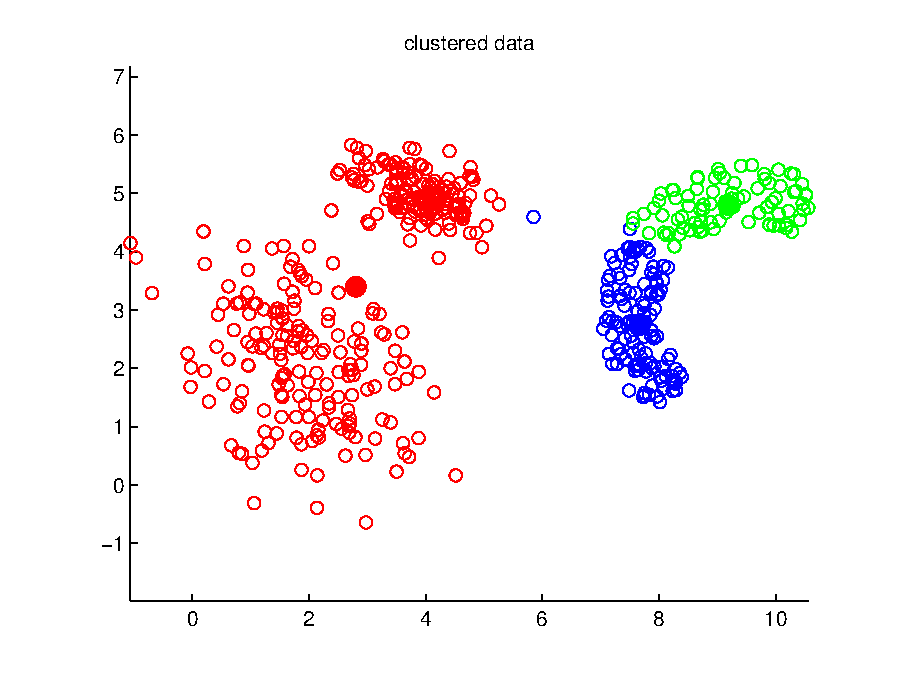
\includegraphics[width=.9\linewidth]{k-means_2}
			\caption{when wrong initialization values are chosen}
			\label{fig:k-means_2}
		\end{subfigure}
		\caption{k-means result}
		\label{fig:fig}
	\end{figure}
	\noindent
%	\\
	3. \textbf{An error-free k-means algorithm implementation should not cluster the second dataset according to the ground truth. Explain why this happens.}\\
	\noindent
	%%%%%%%%%%%%%%%%%%%%%%%%%%%%%%%
	%%% FIGURE 1
	%%%%%%%%%%%%%%%%%%%%%%%%%%%%%%%	
	\begin{figure}[htbp]
		\centering
		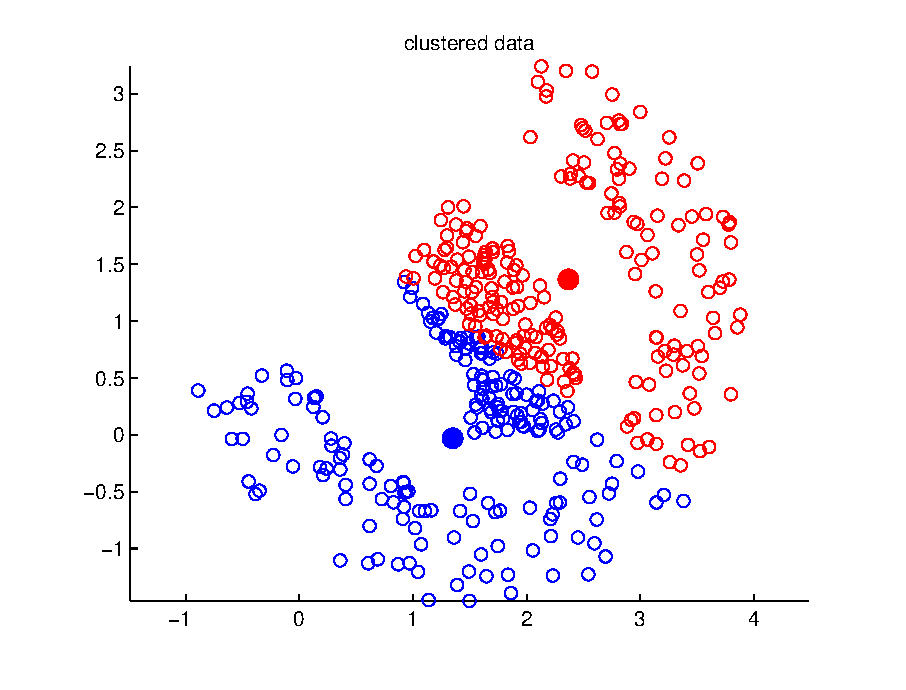
\includegraphics[scale=.7]{dataset2_1}
		\caption{k-means result in dataset 2}
		\label{fig:dataset2}
	\end{figure}
	\\
	\noindent
	K-means algorithm valid on round clusters better. Since the moon shape cluster widely spread on the canvas, it is not possible to separate different clusters into non-touched circles.\\
	%%%%%%%%%%%%%%%%%%%%%%%%%%%%%%%%%%%%%%%%%%%%%%%%%%%%%%%%%%%%%%%%%%%%%%%%%%%%%%%%%%%%%%%%
	%%%%%%   question 3
	%%%%%%%%%%%%%%%%%%%%%%%%%%%%%%%%%%%%%%%%%%%%%%%%%%%%%%%%%%%%%%%%%%%%%%%%%%%%%%%%%%%%%%%%
	\section*{Solution of question 3}
	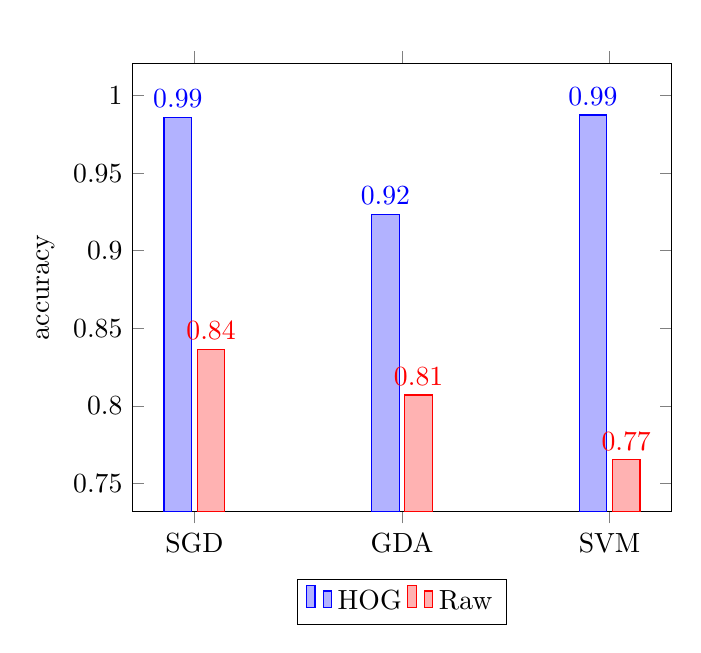
\begin{tikzpicture}
	\centering
	\begin{axis}[
	title={\textbf{}},
	ybar,
	enlargelimits=0.15,
	legend style={at={(0.5,-0.15)},
		anchor=north,legend columns=-1},
	ylabel={accuracy},
	symbolic x coords={SGD,GDA,SVM},
	xtick=data,
	nodes near coords,
	nodes near coords align={vertical},
	]
	\addplot coordinates {(SGD,0.985956) (GDA,0.923473) (SVM,0.987500)};
	\addplot coordinates {(SGD,0.836268) (GDA,0.807026) (SVM,0.765226)};
	\legend{HOG, Raw}
	\end{axis}
	\end{tikzpicture}
	\noindent
	\\
	1. \textbf{Before running the code, what results do you expect to see? What will be the effect of dimensionality reduction on the accuracy and on the computational time (for each classifier)?}\\
	\\
	The main idea of PCA is to reduce data's dimension so that simplify the complexity of calculation.\\
	\\
	Therefore, the expected computational time will reduce with the decreasing of dimensionality reduction. And among these three algorithms, SVM benefits most from this reduction.\\
	\\
	2. \textbf{Use the raw pixels as a feature representation. Compare the learning algorithms we studied so far (logistic regression, GDA, SVM). What is a good choice for $m$ in each case?}\\
	\\
	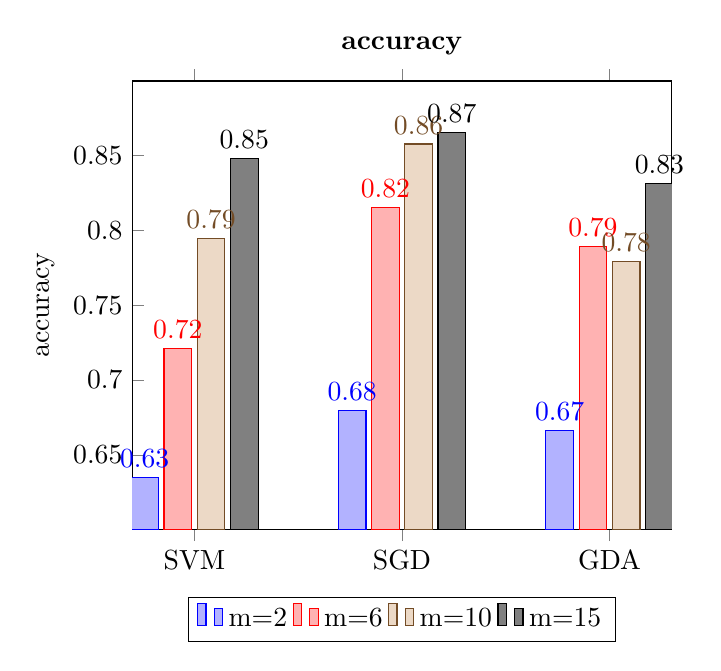
\begin{tikzpicture}
	\centering
	\begin{axis}[
	title={\textbf{accuracy}},
	ybar,
	enlargelimits=0.15,
	legend style={at={(0.5,-0.15)},
		anchor=north,legend columns=-1},
	ylabel={accuracy},
	symbolic x coords={SVM,SGD,GDA},
	xtick=data,
	nodes near coords,
	nodes near coords align={vertical},
	]
	\addplot coordinates {(SVM,0.634921) (SGD,0.679554) (GDA,0.666328)};
	\addplot coordinates {(SVM,0.721165) (SGD,0.815223) (GDA,0.789232)};
	\addplot coordinates {(SVM,0.794402) (SGD,0.857560) (GDA,0.779268)};
	\addplot coordinates {(SVM,0.848136) (SGD,0.865112) (GDA,0.831114)};
	\legend{m=2,m=6,m=10,m=15}
	\end{axis}
	\end{tikzpicture}
	\noindent
	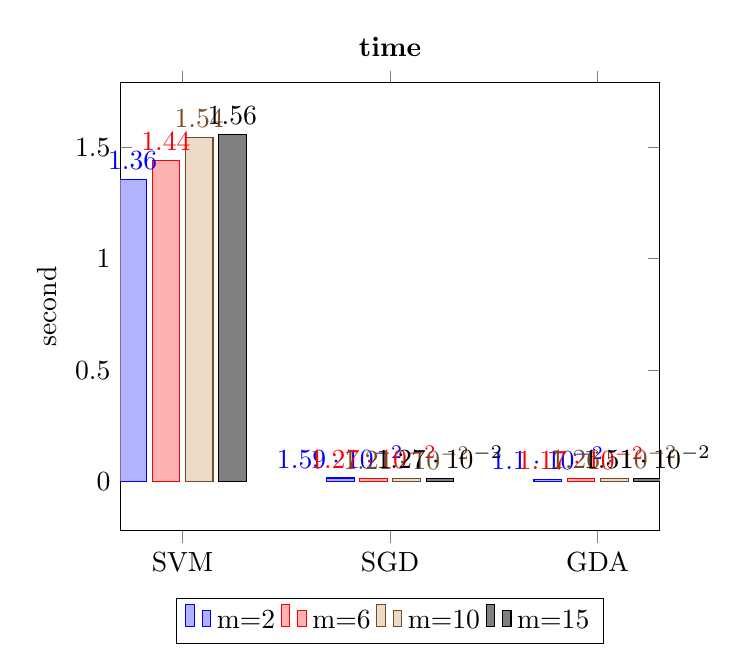
\begin{tikzpicture}
	\centering
	\begin{axis}[
	title={\textbf{time}},
	ybar,
	enlargelimits=0.15,
	legend style={at={(0.5,-0.15)},
		anchor=north,legend columns=-1},
	ylabel={second},
	symbolic x coords={SVM,SGD,GDA},
	xtick=data,
	nodes near coords,
	nodes near coords align={vertical},
	]
	\addplot coordinates {(SVM,1.356275) (SGD,0.015911) (GDA,0.011016)};
	\addplot coordinates {(SVM,1.442150) (SGD,0.012687) (GDA,0.011745)};
	\addplot coordinates {(SVM,1.544691) (SGD,0.012071) (GDA,0.012602)};
	\addplot coordinates {(SVM,1.558624) (SGD,0.012707) (GDA,0.015101)};
	\legend{m=2,m=6,m=10,m=15}
	\end{axis}
	\end{tikzpicture}
	\\
	\noindent
	\\
	When using raw pixel as feature representation, the computational time increases greatly with M increases. In the case of SGD and GDA, the computational time increases not much when using greater M. While SVM's computational time increases greatly if greater M is used.\\
	\\
	In my case, M values range from 2 to 15 are applied. When using SGD and GDA, when greater M is, the performance is better. However in case of SVM, the accuracy to computational time ratio is used as criteria. So M=15 is the best.\\
	\\
	3. \textbf{Compare the result you get on the HOG features with the result on the raw pixels. If we fix an accuracy level for the classifier, which feature representation (between HOG and raw pixels) requires fewer principal components?}\\
	\\
	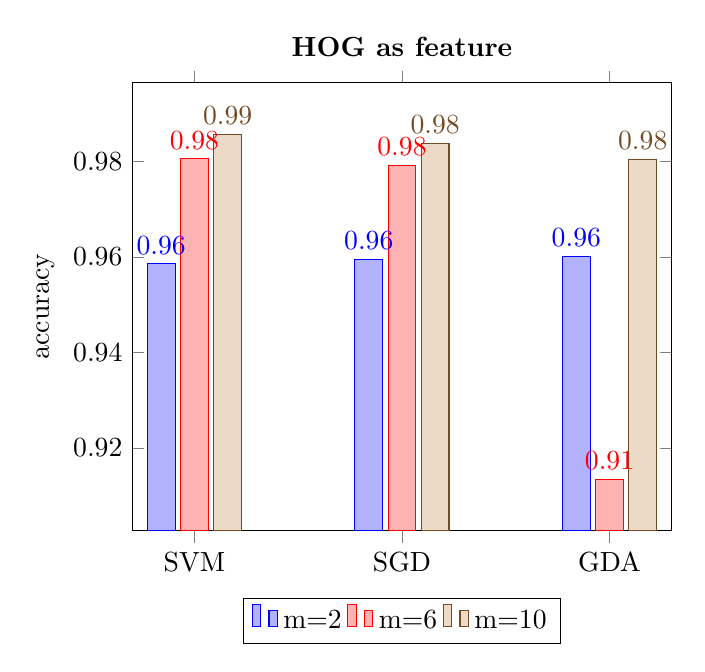
\begin{tikzpicture}
	\centering
	\begin{axis}[
	title={\textbf{HOG as feature}},
	ybar,
	enlargelimits=0.15,
	legend style={at={(0.5,-0.15)},
		anchor=north,legend columns=-1},
	ylabel={accuracy},
	symbolic x coords={SVM,SGD,GDA},
	xtick=data,
	nodes near coords,
	nodes near coords align={vertical},
	]
	\addplot coordinates {(SVM,0.958517) (SGD,0.959446) (GDA,0.960088)};
	\addplot coordinates {(SVM,0.980478) (SGD,0.979065) (GDA,0.913495)};
	\addplot coordinates {(SVM,0.985649) (SGD,0.983704) (GDA,0.980353)};
	\legend{m=2,m=6,m=10}
	\end{axis}
	\end{tikzpicture}
	\\
	\noindent
	\\
	From the measured results, when accuracy is fixed (98\%), the SVM needs smallest principle components m=6. SGD needs m=10 and GDA needs m=10 respectively.\\
	% --------------------------------------------------------------
	%     You don't have to mess with anything below this line.
	% --------------------------------------------------------------
	
\end{document}
